% !TEX root = ../main.tex
Um die Digitalisierung der deutschen Krankenhauslandschaft im internationalem Vergleich einzuordnen, werden hier Deutschland, Österreich und die deutschsprachige Schweiz miteinander in Bezug gesetzt. Datengrundlage des Vergleichs ist der IT-Report Gesundheitswesen 2020 der Hochschule Osnabrück.
\subsection{IT-Report Gesundheitswesen 2020}
Für diesen Ländervergleich wird der IT-Report Gesundheitswesen 2020 herangezogen, in welchem nicht nur deutsche Krankenhäuser, sondern auch Krankenhäuser aus Österreich und der Schweiz, zum Thema Digitalisierung befragt wurden. Die Befragung fand im Jahr 2017 vom 1.7. bis zum 14.12. statt und bestand aus 87 Fragen, gerichtet an ärztliche und pflegerische Direktoren. Insgesamt wurden 2421 Krankenhäuser angeschrieben, davon 1951 in Deutschland, 260 in Österreich und 211 aus der deutschsprachigen Schweiz \parencite{huebner2020}. Laut statista gab es im Jahr 2017 1942 Krankenhäuser in Deutschland\footnote{https://de.statista.com/statistik/daten/studie/2617/umfrage/anzahl-der-krankenhaeuser-in-deutschland-seit-2000/}, 271 Krankenhäuser in Österreich\footnote{https://de.statista.com/statistik/daten/studie/298568/umfrage/oesterreic-hanzahl-der-krankenhaeuser-seit-1985/} und 281 Krankenhäuser in der Schweiz\footnote{https://de.statista.com/statistik/daten/studie/306939/umfrage/anzahl-der-krankenhaeuser-in-der-schweiz/}. Es wurden also fast alle Krankenhäuser in den drei Regionen angeschrieben. Antworten kamen aus 608 Krankenhäusern, davon 492 aus Deutschland (Rücklaufquote $25,2\%$), 49 aus Österreich ($18,8\%$), 67 aus der deutschsprachigen Schweiz ($31,8\%$). Eine Übersicht über diese Zahlen befindet sich in Tabelle \ref{tab:anzahl-krankenhaeuser}.\\

Von den 87 Fragen ermitteln 37 den Stand der Digitalisierung in den klinischen Prozessen und 50 untersuchen einzelne IT-Funktionen, die elektronische Patientenakte und das IT-Management.\\
\begin{table}[ht]
\begin{center}
	\begin{tabular}{l|c|c|c|l}
		&Angeschrieben&\parbox[c]{13ex}{\centering Krankenhäuser\\ insgesamt}&Antworten&Rücklaufquote\\
		\hline
		Deutschland&$1951$&$1942$&$608$&$25,2\%$\\
		Österreich&$260$&$271$&$49$&$18,8\%$\\
		Schweiz&$211$&$281$&$67$&$31,8\%$\\
	\end{tabular}
\end{center}
\caption{Übersicht über befragte Krankenhäuser}	
\label{tab:anzahl-krankenhaeuser}
\end{table}\\
In der Studie wird kein intensiver wertender Vergleich durchgeführt. Aufgrund dessen wird in dieser Arbeit eine eigene Methodik entwickelt.
\subsection{Methodik}
	Da der IT-Report 2020 keinen quantitativen Vergleich der Ergebnisse angibt, wird eine eigene Vergleichsmethodik entwickelt. Die Daten liegen nicht in Rohform vor und werden deshalb manuell in eine Tabellenform zurückgeführt. Für die Bewertung wird für jede Frage das Land ermittelt, welches am besten abgeschnitten hat. Die Ergebnisse der Befragung werden anhand vier verschiedenen Darstellungen vorgestellt, die unterschiedlich ausgelesen und bewertet werden müssen. Es gibt \textit{einfache Balkendiagramme}, \textit{Balkendiagramme mit mehreren Teilfragen}, die mit ja oder nein beantwortet wurden, \textit{gestapelte Balkendiagramme} und \textit{Boxplots}.
	\vspace{\parheadvspace}\\
	\textbf{Einfache Balkendiagramme}\\
	Für Balkendiagramme werden die Werte der einzelnen Balken in eine Tabelle übernommen. Um die Fragen miteinander zu vergleichen, wird entschieden, welche Antworten einen positiven Effekt auf Digitalisierung anzeigen. Die Prozentwerte dieser Antworten werden dann addiert und das Land mit dem höchsten Wert wird als an Platz 1 gesetzt.
	\vspace{\parheadvspace}\\
	\textbf{Balkendiagramme mit mehreren Teilfragen}\\
	Für jede Teilfrage wird die positive Antwort aufgeschrieben. Fragen, die in dieser Darstellung präsentiert werden, zielen darauf ab, welche IT-Funktionen, Geräte o.Ä. im Krankenhaus zur Verfügung stehen. Dabei wird nur nach der Existenz gefragt. Es wird angenommen, dass die Existenz immer positiv im Hinblick auf die Digitalisierung zu bewerten ist. Unter dieser Annahme wird für jede Teilfrage ermittelt, welches Land am besten abschneidet und die Frage insgesamt dem Land zugeschrieben, das am meisten Teilfragen gewonnen hat. Bei einem Gleichstand von zwei Ländern wird die Frage für Beide gewertet. Bei einem Gleichstand von allen drei Ländern wird die Frage vom Vergleich ausgeschlossen.
	\vspace{\parheadvspace}\\
	\textbf{Gestapelte Balkendiagramme}\\
	Bei dieser Darstellung haben die Autoren der Studie aus optischen Gründen Angaben unter 10\% nicht als Zahl angezeigt \parencite[298]{huebner2020}. Bei einer hohen Anzahl an Antworten (einem hohen $n$) werden die Werte in diesen Fällen geschätzt. Bei einer kleinen Anzahl an Antworten ($n<50$), ist die Anzahl der möglichen Werte so gering, dass der genaue Wert ermittelt werden kann. Auch hier besteht jede Frage aus mehreren Teilfragen. Diese werden wie bei den simpleren Balkendiagrammen einzeln einem Land gutgeschrieben und das Land mit den meisten gewonnenen Teilfragen wird als gesamthafter Gewinner der Frage gewertet.\\

	Die Antwortmöglichkeiten auf die Teilfragen haben hier immer eine klare bewertende Reihenfolge. Es geht entweder um Zustimmung mit einer Aussage (\glqq Stimme überhaupt nicht zu\grqq{ }bis \glqq Stimme voll zu\grqq) oder um die Durchdringung einer IT-Funktion (0\%, unter 50\%, über 50\% oder 100\%). \glqq Weiß nicht\grqq{ }wird ignoriert, da diese Antwort nicht klar bewertet werden kann. Sie wird somit genauso behandelt, wie eine nicht vorhandene Antwort. Jede dieser Antwortmöglichkeiten wird nun einer Wertung von -2 bis 2 zugeschrieben. Jede Wertung wird mit dem entsprechenden Prozentwert multipliziert und dann aufsummiert. Dem Land mit der höchsten Summe wird die Teilfrage gutgeschrieben.
%Papi fragt, warum "Weiß nicht" ignoriert wird.
	\vspace{\parheadvspace}\\
	\textbf{Boxplots}\\
	Boxplots haben eine sehr hohe Informationsdichte, die allerdings schwer zu vergleichen ist. Daher werden hier nur die Mediane notiert und miteinander verglichen. Wie bei den vorherigen beiden Darstellungen, gibt es pro Frage mehrere Teilfragen, die ein Land einzeln für sich entscheiden kann. Die gewonnen Teilfragen werden zusammengezählt und die Frage dem Land zugerechnet, das am meisten Teilfragen gewonnen hat.\\

	Schlussendlich werden für jedes Land die Anzahl der gewonnenen Fragen berechnet. Zusätzlich werden Zwischensummen für die einzelnen klinischen Prozesse gebildet. Jede Frage wird gleich gewichtet. 

% \begin{itemize}
% 	\item Ablesemethodik
% 	\begin{itemize}
% 		\item Bei gestapelten Säulen wurden Werte unter 10\% nicht dazu geschrieben, deshalb wurden sie für große n geschätzt. Für kleine Anzahl der Grundgesamtheit konnten die fehlenden Werte ermittelt werden, da nicht viele in Frage kamen.
% 	\end{itemize}
% 	\item Einfache Vergleichsmethodik
% 	\item Fokus: Universitätsmedizin wird ignoriert
% 	\item Für jede Frage gibt es einen Gewinner
% 	\begin{itemize}
% 		\item Bei Gleichstand von 2 Ländern zählen beide als Gewinner
% 	\end{itemize}
% 	\item Wann ist jemand ein Gewinner?
% 	\item \textit{Weiß nicht} wird ignoriert
% 	\begin{itemize}
% 		\item wird indirekt neutral oder negativ bewertet
% 	\end{itemize}
% 	\item bsp Papier einscannen: Geht das direkt in ne datenbank? Wahrschienlich nicht
% 	\begin{itemize}
% 		\item Boxplots
% 		\item Boxplots erklären \parencite[44]{kronthaler2016}
% 		\begin{itemize}
% 			\item Größter Median > größtes oberstes Quartil > größter oberster Whisker
% 			\item evtl. wie bei Güte der Informationsversorgung
% 		\end{itemize}
% 		\item Einfache Säulen mit wenig Antwortmöglichkeiten
% 		\begin{itemize}
% 			\item Summe der Antworten, die Digitalisierung anzeigen
% 			\item Größte Summe gewinnt
% 		\end{itemize}
% 		\item Ja/Nein Säulen mit vielen Kategorien
% 		\begin{itemize}
% 			\item Jede Kategorie gewinnt einzeln
% 			\item Land mit den meisten Kategorien gewinnt Frage
% 			\item Was passiert wenn Länder gleich viele Kategorien gewinnen
% 		\end{itemize}
% 		\item Gestapelte Säulen
% 		\item Güte der Informationsversorgung (Schweiz hat bei Aufnahme nicht teilgenommen)
% 		\begin{itemize}
% 			\item Antworten werden gewichtet
% 			\item ''Stimme überhaupt nicht zu'' = -2 bis ''Stimme voll zu'' = +2
% 			\item multipliziert mit Prozent der Stimmen und dann addiert
% 			\item Scores für alle Kategorien summieren
% 			\item höchster Score gewinnt
% 		\end{itemize}
% 	\end{itemize}
% 	\item Jeder Prozess wird einzeln betrachtet
% 	\item Für jede Frage wird entschieden was einen Digitalisierungsfortschritt darstellt
% \end{itemize}
\subsection{Gegenüberstellung der Länder}

Bei der gewählten Methodik ist zwar erkennbar welches Land die meisten Fragen gewonnen hat, aber nicht wie deutlich der Vorsprung gegenüber den anderen Ländern ist. Diese Ergebnisse geben somit nur eine vergleichende und keine qualitative Übersicht. Die Gegenüberstellung erfolgt nach der Struktur, die im IT-Report Gesundheitswesen 2020 vorgegeben ist. So werden zuerst die klinischen Prozesse betrachtet und anschließend verschiedene IT-Funktionstypen und das IT-Management. Eine Übersicht über die Ergebnisse befindet sich in Abbildung \ref{fig:laender_ergebnisse}.
\begin{figure}
	\centering
	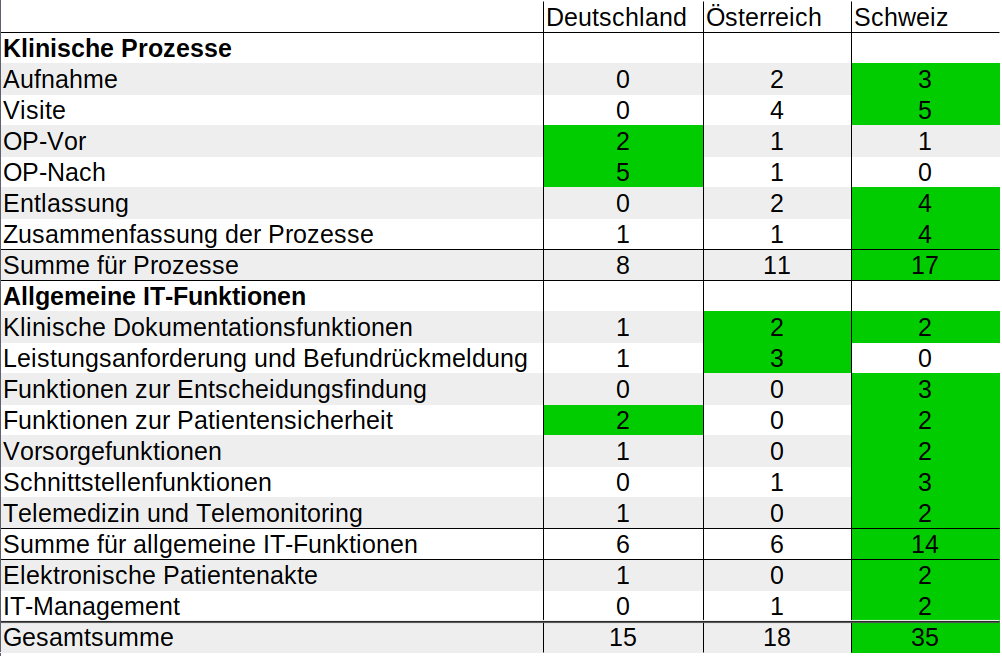
\includegraphics[width=0.7\textwidth]{Bilder/laendervergleich_ergebnisse.png}
	\caption{Ergebnisse des Ländervergleichs. Die Gewinner einer Kategorie sind grün markiert}
	\label{fig:laender_ergebnisse}
\end{figure}
\vspace{\parheadvspace}\\
\textbf{Klinische Prozesse}\\
In den Prozessen Aufnahme, Visite und Entlassung ist die Schweiz Vorreiter, während in den Unterstützungsprozessen des OPs Deutschland führt. Es scheint, dass die externen Schnittstellen, Aufnahme und Entlassung, in Österreich und der Schweiz deutlich digitaler sind als in Deutschland. In der Visite zeigt sich vor allem eine höhere Verfügbarkeit von mobilen Geräten zum Zugriff auf Patientendaten und damit verbunden eine weitere Verbreitung von WLAN in Österreich und der Schweiz im Vergleich zu Deutschland. Daten im OP-Verlauf stehen in Deutschland jedoch deutlich häufiger in elektronischer Form bereit und die Informationsgüte ist höher, was sich am guten Abschneiden in der OP-Vorbereitung widerspiegelt. Bei der OP-Nachbereitung ergibt sich ein ähnliches Bild. Da OP-Daten in deutschen Krankenhäusern häufiger elektronisch verfügbar sind, können sie auch einfacher auf die Stationen übernommen werden. Die Zufriedenheit mit dem IT-Einsatz in den fünf Prozessen ist in der Schweiz am höchsten. Auch die Verfügbarkeit wesentlicher Patientendaten wird von schweizer Klinikern am besten eingeschätzt.
\vspace{\parheadvspace}\\
\textbf{Weitere IT-Funktionen}\\
Das Bild von der Schweiz als Vorreiter verdeutlicht sich bei der Betrachtung ausgewählter IT-Funktionen, die nicht klar einem klinischen Prozess zugeordnet werden. Lediglich bei \textit{Leistungsanforderung und Befundrückmeldung} schneidet Österreich besser ab. Während \textit{Funktionen zur Entscheidungsfindung} in Krankenhäusern aller drei Länder selten eingesetzt werden, sind diese in der Schweiz dennoch am verbreitetsten.
\vspace{\parheadvspace}\\
\textbf{Elektronische Patientenakte}\\
Eine elektronische Patientenakte (ePA) steht in nur rund der Hälfte aller deutschen und österreichischen Krankenhäuser zur Verfügung. In der deutschsprachigen Schweiz hingegen haben über drei Viertel aller Krankenhäuser eine ePA implementiert. Wenn ein Krankenhaus eine ePA nutzt, wird sie meistens im allen relevanten Einheiten genutzt.
\vspace{\parheadvspace}\\
\textbf{IT-Management}\\
Die Zufriedenheit mit dem IT-Support ist in Österreich und der Schweiz höher als in Deutschland. Zusätzlich ist die Integration der IT-Abteilung in der Schweiz am besten, wo es eine hohe Beteiligung des klinischen Personals an IT-Angelegenheiten gibt.\\

Im Allgemeinen ergibt sich bei Betrachtung der Daten des IT-Report Gesundheitswesen 2020 ein klares Bild: Die deutschsprachige Schweiz ist in Sachen Digitalisierung den andern Ländern vorraus. Deutschland bildet das Schlusslicht. Österreich befindet sich im Mittelfeld, ist aber deutlich näher an Deutschland als an der Schweiz. Das entspricht auch der Einschätzung in der Zusammenfassung des Reports \parencite[29]{huebner2020}.

\subsection{Weitere Länder}
Für eine breitere Übersicht über den internationalen Stand der Digitalisierung an Krankenhäusern wird hier eine Übersicht des Schnitts der EMRAM-Werte ausgewählter Länder von 2011 bis 2017 (siehe Abbildung \ref{fig:andere_laender}) aus \cite{Stephani2019} herangezogen. Eine Übersicht darüber wie diese Werte ermittelt werden, befindet sich in Kapitel \ref{sec:EMRAM}. Man kann erkennen, dass Deutschland und Österreich mit einem Mittelwert von $2,3$ auf einem ähnlichen Niveau liegen, welches wiederum deutlich unter dem europäischen Durchschnitt von $3,6$ liegt. An dieser Stelle sollte erwähnt werden, dass sich 167 deutsche Krankenhäuser über den Zeitraum zertifizieren ließen; in Österreich waren es nur 18. Führende Länder in Europa sind die Niederlande ($n=36$) und Dänemark ($n=24$), mit einem Schnitt von $4,8$ respektive $5,4$. Die Türkei ($n=682$), das Vereinigte Königreich ($n=105$) und Spanien ($n=156$) liegen nahe am europäischen Mittel.
\begin{figure}[ht]
	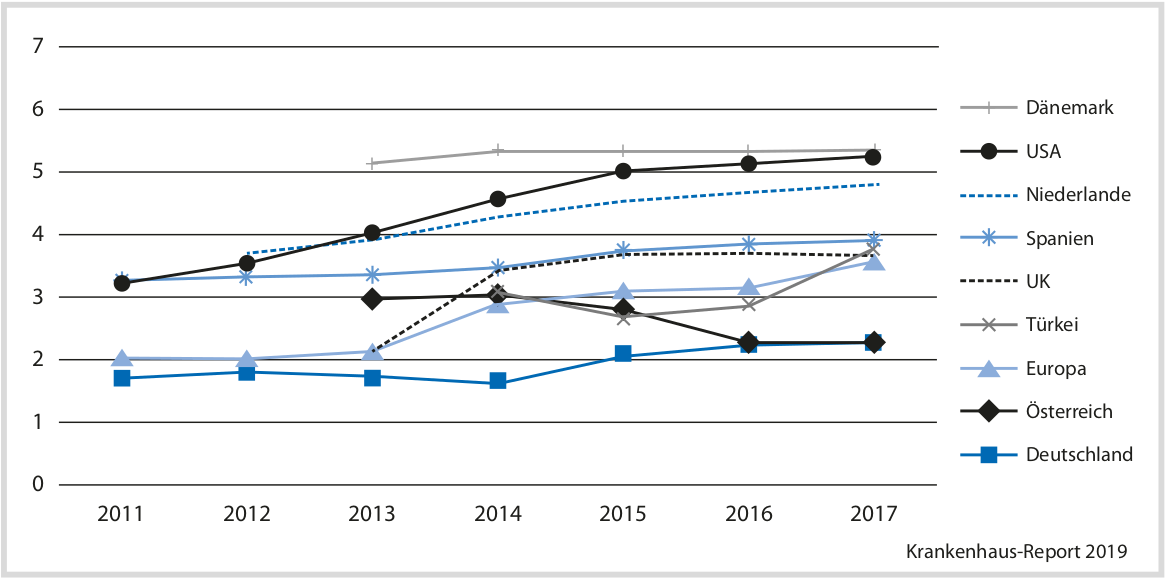
\includegraphics[width=0.95\textwidth]{Bilder/laendervergleich_EMRAM_Stephani_2019.png}
	\caption{Durchschnittliche EMRAM-Werte in ausgewählten Regionen seit 2011 \parencite{Stephani2019}}
	\label{fig:andere_laender}
\end{figure}
